% $Header: /cvsroot/latex-beamer/latex-beamer/solutions/generic-talks/generic-ornate-15min-45min.en.tex,v 1.5 2007/01/28 20:48:23 tantau Exp $

\documentclass{beamer}
%\documentclass[handout]{beamer}
%\usepackage{pgfpages}
%\pgfpagesuselayout{2 on 1}[a4paper,border shrink=5mm]

\newcommand{\Href}[1]{\htmladdnormallink{#1}{#1}}
\newcommand\Qt{\"{}}                   % Double quotes...
\newcommand\Bs{\char '134}             % Backslash character for the \tt font
\newcommand\Or{\texttt{|}\,\,}         % Logical Or
\newcommand\BPipe{\,\rule[-.8ex]{1.8pt}{2.6ex}\,}
\newcommand\BOr{\BPipe}    % Logical Or (bold)
\newcommand\Nl{'{\Bs}0'}               % Nul character in C ('\0')
\newcommand\rarrow{$\longrightarrow$ } % A rightarrow


% This file is a solution template for:

% - Giving a talk on some subject.
% - The talk is between 15min and 45min long.
% - Style is ornate.


\mode<presentation>
{
  \usetheme{Fdc}
  % or ...

  %\setbeamercovered{transparent}
  \setbeamercovered{invisible}
  % or whatever (possibly just delete it)
}


\usepackage[english]{babel}

\usepackage[latin1]{inputenc}

\usepackage{times}
\usepackage[T1]{fontenc}


\title[Wavelet-Based Image Search] % (optional, use only with long paper titles)
{A Wavelet-Based, Image-Property-Based Image Search Engine}


\author{Martin~Dietze}

\institute{Freiheit.com Technologies}

\date[Short Occasion] % (optional)
{May 14, 2009 / Hacker Talk}

\subject{Talks}
% This is only inserted into the PDF information catalog. Can be left
% out. 



% If you have a file called "university-logo-filename.xxx", where xxx
% is a graphic format that can be processed by latex or pdflatex,
% resp., then you can add a logo as follows:

\pgfdeclareimage[height=0.3cm]{freiheit-logo}{freiheit-logo}
\logo{\pgfuseimage{freiheit-logo}}



\def\RImageSize{0.2\textwidth}
\def\RImageSpace{\hspace{1cm}}


\begin{document}

\begin{frame}
  \titlepage
\end{frame}

\begin{frame}{Outline}
  \tableofcontents
  % You might wish to add the option [pausesections]
\end{frame}


% - Exactly two or three sections (other than the summary).
% - At *most* three subsections per section.
% - Talk about 30s to 2min per frame. So there should be between about
% 15 and 30 frames, all told.

\section{Introduction}

\begin{frame}{/ Introduction / Requirements}
  % - A title should summarize the slide in an understandable fashion
  % for anyone how does not follow everything on the slide itself.

  \begin{itemize}
  \item Find images from a database
  \item Based on image features / similarity
  \item Matches need only be ``as good as possible''
  \item Query against scanned or hand-drawn images
  \end{itemize}

  \pause
  \begin{itemize}
  \item Fast
  \item Modest memory footprint
  \item Web interface
  \end{itemize}

  \pause
  \begin{itemize}
  \item Idea: Fast Multiresolution Image Querying \emph{[Jacobs95]}
  \item Wavelet-based approach
  \end{itemize}
\end{frame}

\section{Wavelets}

\begin{frame}{/ Wavelets / Basics}

  \begin{itemize}
  \item ``Small Waves'' repeatedly applied on data in different scales
  \item \emph{Multiresolutional} view on data
  \item Change of basis
  \item Combined space / frequency domain representation
  \end{itemize}

  \pause
  \begin{itemize}
  \item \emph{Wavelet Function}: $\psi_\lambda (x)$ with $\psi$ from a function
    space $\cal F$,\\
    $x$ from a spatial domain $X$ and $\lambda$ from an index domain $\Lambda$.
  \item And, accordingly, \emph{Scaling Function}:  $\phi_\lambda (x)$  
  \end{itemize}
\end{frame}

\begin{frame}{/ Wavelets / Examples}

  \begin{figure}[hbt]
    \begin{center}
      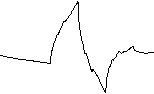
\includegraphics[width=\RImageSize]{daubechies-d4-wavelet.jpg}
      \RImageSpace
      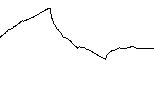
\includegraphics[width=\RImageSize]{daubechies-d4-scaling.jpg}
      \caption{The Daubechies D4 Wavelet and Scaling Functions}
    \end{center}
  \end{figure}

  \pause
  \begin{figure}[hbt]
    \begin{center}
      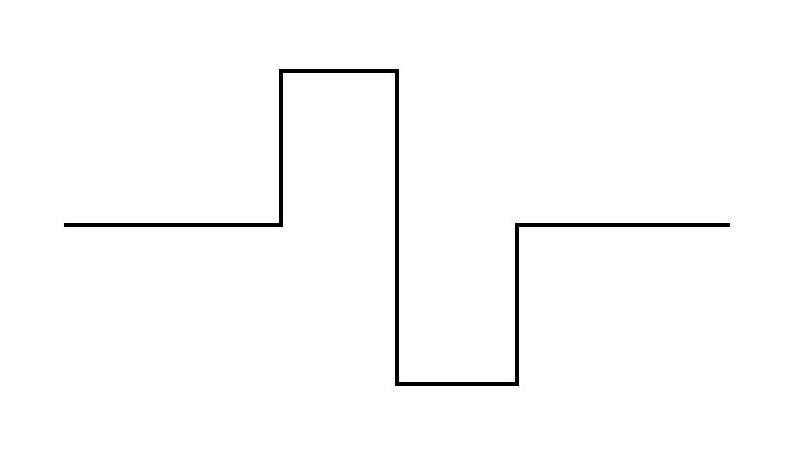
\includegraphics[width=\RImageSize]{haar-wavelet.jpg}
      \RImageSpace
      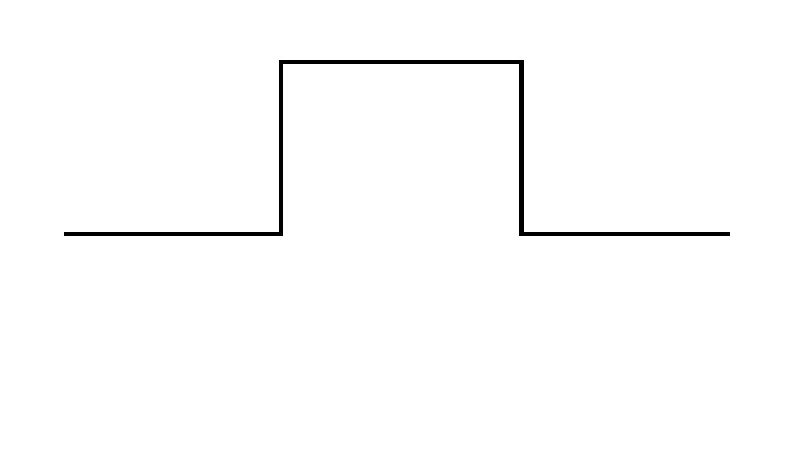
\includegraphics[width=\RImageSize]{haar-scaling.jpg}
      \caption{The Haar Wavelet and Scaling Functions}
    \end{center}
  \end{figure}

\end{frame}

\begin{frame}{/ Wavelets / Images}

  \begin{figure}[hbt]
    \begin{center}
      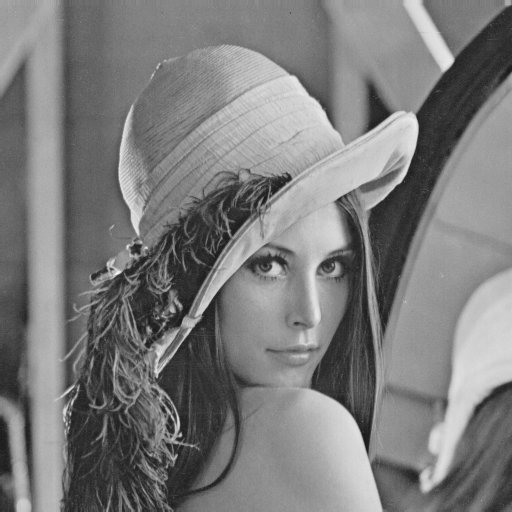
\includegraphics[width=\RImageSize]{lena512.jpg}
      \RImageSpace
      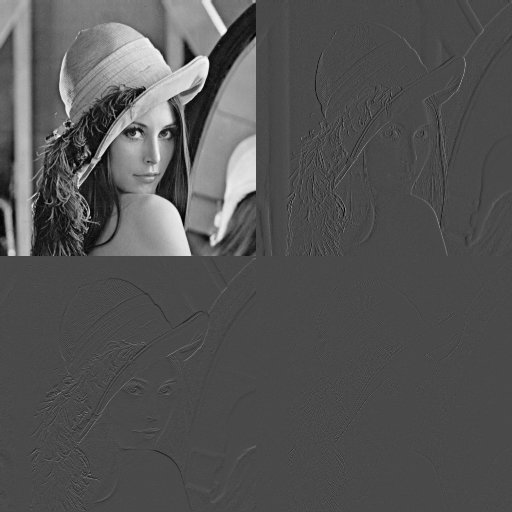
\includegraphics[width=\RImageSize]{lena-1step.jpg}
    \end{center}
  \end{figure}
  \begin{figure}[hbt]
    \begin{center}
      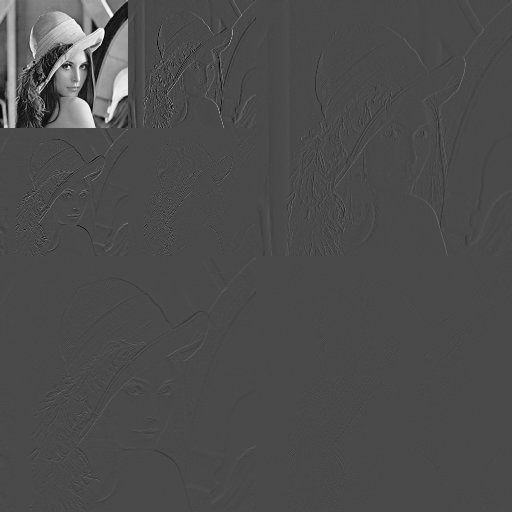
\includegraphics[width=\RImageSize]{lena-2step.jpg}
      \RImageSpace
      
\includegraphics[width=\RImageSize]{lena-9step.jpg}
      \caption{Decomposing Lena}
    \end{center}
  \end{figure}

\end{frame}

\section{Algorithm}

\begin{frame}{/ Algorithm / Score Table}

  \begin{itemize}
  \item Transform the image to \emph{YUV} colour space
  \item Perform a full \emph{Haar} Decomposition on the image
  \item For each colour channel:
    \begin{enumerate}
    \item Sort the wavelet coefficients by absolute values
    \item Discard all but the most significant $n$ (parameter) values
    \item Quantise the remaining values to $\pm 1$
    \end{enumerate}
  \end{itemize}

  \pause
  \begin{itemize}
  \item For each colour channel: one \emph{plus} and \emph{minus}
    table
  \item Each table consists of $YX$ ($Y$ rows, $X$ cols) binary arrays 
  \item Each array contains the information whether image $I_n$ contains
    a significant coefficient at position $y, x$\\
    with sign according to its table
  \end{itemize}

\end{frame}

\begin{frame}{/ Algorithm / Matching}

  \begin{itemize}
  \item Same transform and quantisation as for the score table
  \item Init score by sum of weighted differences of the colour channels'
    corresponding overall average values
  \item For each pixel position of each colour channel:
    \begin{enumerate}
    \item If this coefficient $>$ 0, use the \emph{Plus} array,
      else \emph{Minus}
    \item For each image in the array subtract a value (depends on
      subband) if the image has a matching value at that position
    \end{enumerate}
  \item The lower the score value the better the match
  \end{itemize}

\end{frame}

\section{Implementation}

\begin{frame}{/ Implementation / Initial Version}

  \begin{itemize}
  \item C++, libstdc++
  \item My own Wavelet library \emph{[libWavelet]}
  \item Some boost libraries \emph{[boost]}
  \item PostgresQL and a C++ API \emph{[pqxx]}
  \item WT Web Toolkit \emph{[wt]}
    \pause
  \item And: \texttt{M-x viper-mode} :)
  \end{itemize}

    \pause
  \begin{itemize}
  \item Use image IDs as offsets in \emph{plus} and \emph{minus} arrays
  \item One bit per image and array
  \item The Score Table is a \emph{singleton}
  \end{itemize}

\end{frame}

\begin{frame}{/ Implementation / Second Approach to Score Table}

  \begin{itemize}
  \item Quest for better runtime performance
  \item Initial assumption: faster queries, bigger memory footprint
  \item Alternative Score Table \rarrow \emph{OPEN IMPLEMENTATION}\\
    \texttt{ScoreTableFactory::create (/*...*/, SPEED)}\\
    \texttt{ScoreTableFactory::create (/*...*/, SIZE)}\\
  \end{itemize}

  \pause
  \begin{itemize}
  \item In the \emph{plus} and \emph{minus} arrays, store the IDs of
    images which have the right values at the respective locations

    \rarrow More work at setup, fewer comparisons when querying
  \end{itemize}

\end{frame}

\section{Results and Discussion}

\begin{frame}{/Results and Discussion / Comparing the Approaches}

  \begin{itemize}
    \item Experimental Results (610 images, 60 kept coefficients):
      \begin{center}
        \begin{tabular}{|l|r|r|}\hline
          ~ & \texttt{SIZE} & \texttt{SPEED} \\ \hline\hline
          Initial Setup Time & 13.2 sec & 8.2 sec \\ \hline
          Average Query Time & 4.0 ms  & 0.0 ms \\ \hline
          Score Table Size & 29.98 MB  & 6.29 MB \\ \hline
        \end{tabular}
      \end{center}
      \medskip

        \pause
      \item The \texttt{SPEED} variant takes \emph{less} space

        \pause
        \rarrow \texttt{\%s/SIZE/BAD/g}\pause, \texttt{\%s/SPEED/GOOD/g} \pause :)

  \end{itemize}

\end{frame}

\begin{frame}{/ Results and Discussion / Technologies \# 1}

  \begin{itemize}
  \item Wavelet-Lib:
    \begin{itemize}
    \item 26,000 lines of C++ code
    \item Rather old (started in 1994)
    \item No STL, no smart pointers
    \item Prone to memory leaks
    \item Nevertheless well-tested (thanks to \emph{valgrind})
    \end{itemize}
    \pause
  \item Pqxx:
    \begin{itemize}
    \item STL-containers
    \item Insufficient documentation
    \item PostgresQL only
    \item Tedious to use
    \item Better try \emph{hiberlite} or \emph{sqlite} in future!
    \end{itemize}
  \end{itemize}
  
\end{frame}

\begin{frame}{/ Results and Discussion / Technologies \# 2}

  \begin{itemize}
  \item WT:
    \begin{itemize}
    \item Elegant, QT-like API (\rarrow \emph{Signals}, \emph{Slots})
    \item Supports clean separation of model, view, controller
    \item Good CSS support
    \item Good Ajax integration
    \item Very code-based, use of HTML templates is difficult to
      integrate
    \item After little time, productivity felt quite good, a bit like
      \emph{Wicket}
    \end{itemize}
    \pause
  \item Technology which was missing:
    \begin{itemize}
    \item I missed \emph{Spring}; handwritten wiring of services was
      still simple enough, but with increasing size...
    \end{itemize}
  \end{itemize}
  
\end{frame}

\section*{Summary}

\begin{frame}{Summary}

  \begin{itemize}
  \item The image search engine is fast and memory efficient
  \item Results are good on images with few details
  \item Images of landscapes are problematic
  \end{itemize}
  
  \pause
  \vskip0pt plus.5fill
  \begin{itemize}
  \item Future Work
    \begin{itemize}
    \item Rewrite the database backend code and get rid of \emph{pqxx}
    \item More experiments with different weight factors and
      numbers-of-kept-coefficients
    \end{itemize}
    \pause
  \item That's all, folks!
  \end{itemize}
\end{frame}

\section*{References}

\begin{frame}{References}

  \begin{description}
  \item[\textit{[Jacobs95]}] Charles E. Jacobs and Adam Finkelstein and David H. Salesin, \emph{Fast Multiresolution Image Querying}, Computer Graphics \#29, 1995
  \item[\textit{[libWavelet]}] Martin Dietze, \emph{Wavelet library}, \Href{http://herbert.the-little-red-haired-girl.org/en/wavelet/index.html}

  \item[\textit{[boost]}] Various, \emph{Boost libraries}, \Href{http://www.boost.org}

  \item[\textit{[pqxx]}] Various, \emph{Pqxx PostgresQL wrapper}, \Href{http://pqxx.org}

  \item[\textit{[wt]}] Various, \emph{WT Web Toolkit}, \Href{http://www.webtoolkit.eu}
  \end{description}

\end{frame}

\end{document}


